% !TEX root = main.tex
\subsection{2D MRI}
% Alle einzelnen Plots
Bei dem Bildgebungsverfahren von dem 2D-MRI gibt es verschiedene Möglichkeiten, wie hier vorgegangen werden kann. Da im Versuch nur das Bildgebungsverfahren mit dem Gradientenecho benutzt wurde, wird nur dieses explizit erklärt.\\
Aufgrund von der Linearität der Fourietransformation kann nicht nur in 1D ein Bild von Objekten gemacht werden, sondern auch in 2D. Wie dies genau funktioniert, wird im folgenden genauer erläutert.\\
In dem Abschnitt davor wurde darauf eingegangen, wie das 1D-MRI funktioniert. Hierzu muss noch hinzu ergäntzt werden, dass bei dem 1D-MRI eine Frequenz-Kodierung stattgefunden hat. Dies bedeutet, dass bei einem konstanten Gradientenfeld die Zeit verändert wurde und dadurch das Spektrum im Fourieraum entstanden ist. \\
In 2D ist es nun üblich, dass neben der Frequenz-Kodierung auch eine sogenannte Phasen-Kodierung stattfindet. Hierbei wird die Zeit konstant gehalten und der sogenannte Phasengradient $G_p$ wird verändert. Die Zeit $t_{grad}$, während das Gradientenfeld angelegt wird, bleibt hierbei immer gleich. Da jedoch ein Gradientenfeld angelegt ist, führt dies dazu, dass die Spins einen Phasenunterschied erhalten, der abhängig von dem Ort ist. Dies kann mit der folgenden Formel beschrieben werden \cite{Schmidt}:
\begin{align}
    \Delta\Phi(x)= \Delta\omega(x)t=\gamma G_xxt
\end{align}\label{eq:phase}
Indem nun der Gradienten von $-G_{max}$ bis $+G_{max}$ im Phasenraum vermessen wird, ergibt dies im k-Raum eine Linie.\\
Das 2D-MRI funktioniert nun so, dass in eine bestimmte Richtung die Frequenz-Kodierung statt findet. Diese Ebene wird auch als die \textit{read}-Ebene bezeichnet. Das Signal was gemessen wird ist analog zu der 1D-MRI Messung, nur mit dem Unterschied, dass ein zusätzlicher Gradientenpuls angelegt wird. Dieser Puls wird senkrecht zum anderen Gradienten angelegt, sodass dies eine Ebene ergibt. Durch das Anlegen des $G_p$ bekommen die Spins eine Larmorfrequenz, die abhängig vom Ort ist. Dies wird als Phasen-Kodierung bezeichnet. \ref{eq:phase}
Insgesamt werden nun $N_p$ Messungen für die Anzahl der jeweiligen Phasengradienten durchgeführt, wobei jedes mal von $-G_{pmax}$ bis $G_{pmax}$ gemessen wird, um ein 2D-MRI zu erhalten.
\begin{figure}[H]
    \centering
    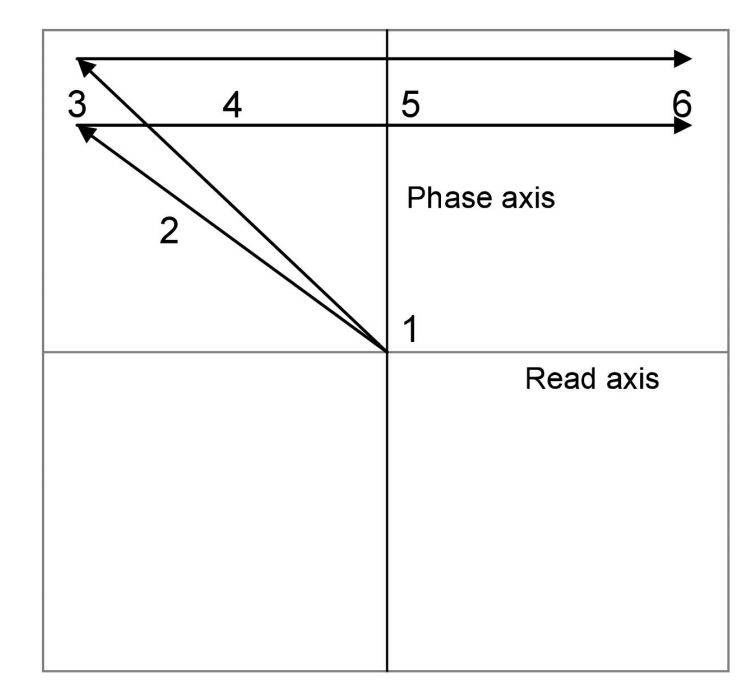
\includegraphics[width = 0.5\textwidth]{Abbildungen/2DMRI.JPG}
    \caption[Veranschaulichter Verlauf des k-Vektors im 2D-MRI]{Hier wird anschaulich ein Verlauf des k-Vektors in der transversalen Ebene dargestellt.\\
    Als erstes wird in Schritt 1 das Signal durch den $90^{\circ}$-Puls in die transversalen Ebene gebracht.\\
    Anschließend wird ein Gradient in negativer \textit{read}-Richtung eingeschaltet. Zusätzlich wird auch der Phasengradient $G_p$ angelegt. Dies bedeutet, dass der k-Vektor in Abhängigkeit von der Zeit durch den \textit{phasen}-und \textit{read}-Raum durchgeht. Dies ist in der Abbildung mit der Nummer 2 markiert, wo der Pfeil vom Ursprung quer nach links oben verläuft.\\
    Im dritten Schritt wird der Phasengradient ausgeschaltet was bedeutet, dass sich der k-Vektor nicht mehr entlang des Phasenraums bewegt und somit nur noch von dem Gradienten in der \textit{read}-Richtung abhängt. Das Vorzeichen von dem \textit{read}-Gradienten wird geflippt, sodass dieser nicht mehr negativ ist sondern positiv. Ab hier findet nun der gleiche Ablauf wie bei der 1D-MRI-Messung statt. Die Larmorfrequenz der Spins werden in Abhängigkeit von der Position gemessen, sodass am Ende eine Linie von Datenpunkte heraus kommt. Diese wurden  zusätzlich noch in Abhängigkeit von der Zeit gemessen. Nachdem eine Linie im k-Raum vermessen wurde, wird der Gradient ausgeschaltet und dieser fängt wieder vom Anfang an. \cite{Schmidt}}
    \label{fig:2DMRIk}
\end{figure}
Durch das Wiederholen der in Abbildung \ref{fig:2DMRIk} dargestellten Messmethode ergibt dies am Ende ein 2D-MRI. Vereinfacht gesagt, ist ein 2D-MRI ein 1D-MRI, welches durch sehr viele Ebenen durchgefahren wurde.

Das Ziel bei dem 2D-MRI ist es nun, welche Auswirkungen unterschiedliche Relaxationszeiten von $T_1$ und $T_2$ auf die Messungen haben und wie diese Kontraste erhöht werden können. Durch Kontrastmittel können unter anderem die Relaxationszeiten der zu untersuchenden Proben verändert werden. Hierbei wird zwischen positiven Relaxationszeiten (diese erhöhen die Intensität der Probe) und negative Kontraste (diese verringern/reduziert die Intensität in der Region) unterschieden.  Diese Kontrastmittel werden dann benutzt, wenn in einer bestimmten Region etwas hervor gehoben werden soll oder schon einen vorhanden Kontrast weiter verstärkt werden soll. \\
Diese Kontrastmittel sind vor allem in der Medizin von großer Bedeutung. Die Kontrastmittel können hierbei von den Patienten Oral eingenommen werden oder werden direkt in die Region gespritz, die von Interesse sind.   
\begin{figure}[H]
\centering
\subcaptionbox{Die Polarisationszeit von $\SI{600}{\milli\second}$ wurde am Anfang gewählt. Dabei handelt es sich um die selbe Zeit wie die $T_1$-Relaxation von der einen Röhre. Hierbei ist in der Abbildung zu sehen, dass es sich um die rechte Röhre handeln muss, da diese bei geringer Polarisationszeit schon eine sehr große Intensität aufweist}
{% GNUPLOT: LaTeX picture with Postscript
\begingroup
  % Encoding inside the plot.  In the header of your document, this encoding
  % should to defined, e.g., by using
  % \usepackage[cp1252,<other encodings>]{inputenc}
  \inputencoding{cp1252}%
  \makeatletter
  \providecommand\color[2][]{%
    \GenericError{(gnuplot) \space\space\space\@spaces}{%
      Package color not loaded in conjunction with
      terminal option `colourtext'%
    }{See the gnuplot documentation for explanation.%
    }{Either use 'blacktext' in gnuplot or load the package
      color.sty in LaTeX.}%
    \renewcommand\color[2][]{}%
  }%
  \providecommand\includegraphics[2][]{%
    \GenericError{(gnuplot) \space\space\space\@spaces}{%
      Package graphicx or graphics not loaded%
    }{See the gnuplot documentation for explanation.%
    }{The gnuplot epslatex terminal needs graphicx.sty or graphics.sty.}%
    \renewcommand\includegraphics[2][]{}%
  }%
  \providecommand\rotatebox[2]{#2}%
  \@ifundefined{ifGPcolor}{%
    \newif\ifGPcolor
    \GPcolorfalse
  }{}%
  \@ifundefined{ifGPblacktext}{%
    \newif\ifGPblacktext
    \GPblacktexttrue
  }{}%
  % define a \g@addto@macro without @ in the name:
  \let\gplgaddtomacro\g@addto@macro
  % define empty templates for all commands taking text:
  \gdef\gplbacktext{}%
  \gdef\gplfronttext{}%
  \makeatother
  \ifGPblacktext
    % no textcolor at all
    \def\colorrgb#1{}%
    \def\colorgray#1{}%
  \else
    % gray or color?
    \ifGPcolor
      \def\colorrgb#1{\color[rgb]{#1}}%
      \def\colorgray#1{\color[gray]{#1}}%
      \expandafter\def\csname LTw\endcsname{\color{white}}%
      \expandafter\def\csname LTb\endcsname{\color{black}}%
      \expandafter\def\csname LTa\endcsname{\color{black}}%
      \expandafter\def\csname LT0\endcsname{\color[rgb]{1,0,0}}%
      \expandafter\def\csname LT1\endcsname{\color[rgb]{0,1,0}}%
      \expandafter\def\csname LT2\endcsname{\color[rgb]{0,0,1}}%
      \expandafter\def\csname LT3\endcsname{\color[rgb]{1,0,1}}%
      \expandafter\def\csname LT4\endcsname{\color[rgb]{0,1,1}}%
      \expandafter\def\csname LT5\endcsname{\color[rgb]{1,1,0}}%
      \expandafter\def\csname LT6\endcsname{\color[rgb]{0,0,0}}%
      \expandafter\def\csname LT7\endcsname{\color[rgb]{1,0.3,0}}%
      \expandafter\def\csname LT8\endcsname{\color[rgb]{0.5,0.5,0.5}}%
    \else
      % gray
      \def\colorrgb#1{\color{black}}%
      \def\colorgray#1{\color[gray]{#1}}%
      \expandafter\def\csname LTw\endcsname{\color{white}}%
      \expandafter\def\csname LTb\endcsname{\color{black}}%
      \expandafter\def\csname LTa\endcsname{\color{black}}%
      \expandafter\def\csname LT0\endcsname{\color{black}}%
      \expandafter\def\csname LT1\endcsname{\color{black}}%
      \expandafter\def\csname LT2\endcsname{\color{black}}%
      \expandafter\def\csname LT3\endcsname{\color{black}}%
      \expandafter\def\csname LT4\endcsname{\color{black}}%
      \expandafter\def\csname LT5\endcsname{\color{black}}%
      \expandafter\def\csname LT6\endcsname{\color{black}}%
      \expandafter\def\csname LT7\endcsname{\color{black}}%
      \expandafter\def\csname LT8\endcsname{\color{black}}%
    \fi
  \fi
    \setlength{\unitlength}{0.0500bp}%
    \ifx\gptboxheight\undefined%
      \newlength{\gptboxheight}%
      \newlength{\gptboxwidth}%
      \newsavebox{\gptboxtext}%
    \fi%
    \setlength{\fboxrule}{0.5pt}%
    \setlength{\fboxsep}{1pt}%
\begin{picture}(7200.00,5040.00)%
    \gplgaddtomacro\gplbacktext{%
    }%
    \gplgaddtomacro\gplfronttext{%
      \csname LTb\endcsname%%
      \put(936,688){\makebox(0,0){\strut{}$0$}}%
      \put(1824,688){\makebox(0,0){\strut{}$20$}}%
      \put(2712,688){\makebox(0,0){\strut{}$40$}}%
      \put(3600,688){\makebox(0,0){\strut{}$60$}}%
      \put(4488,688){\makebox(0,0){\strut{}$80$}}%
      \put(5376,688){\makebox(0,0){\strut{}$100$}}%
      \put(6264,688){\makebox(0,0){\strut{}$120$}}%
      \put(3600,358){\makebox(0,0){\strut{}Y in $\si{\milli \meter}$}}%
      \put(700,938){\makebox(0,0)[r]{\strut{}$0$}}%
      \put(700,1502){\makebox(0,0)[r]{\strut{}$20$}}%
      \put(700,2066){\makebox(0,0)[r]{\strut{}$40$}}%
      \put(700,2630){\makebox(0,0)[r]{\strut{}$60$}}%
      \put(700,3194){\makebox(0,0)[r]{\strut{}$80$}}%
      \put(700,3758){\makebox(0,0)[r]{\strut{}$100$}}%
      \put(700,4322){\makebox(0,0)[r]{\strut{}$120$}}%
      \put(238,2630){\rotatebox{-270}{\makebox(0,0){\strut{}Z in $\si{\milli \meter}$}}}%
      \put(6795,938){\makebox(0,0)[l]{\strut{}$0$}}%
      \put(6795,1421){\makebox(0,0)[l]{\strut{}$5000$}}%
      \put(6795,1904){\makebox(0,0)[l]{\strut{}$10000$}}%
      \put(6795,2388){\makebox(0,0)[l]{\strut{}$15000$}}%
      \put(6795,2871){\makebox(0,0)[l]{\strut{}$20000$}}%
      \put(6795,3355){\makebox(0,0)[l]{\strut{}$25000$}}%
      \put(6795,3838){\makebox(0,0)[l]{\strut{}$30000$}}%
      \put(6795,4322){\makebox(0,0)[l]{\strut{}$35000$}}%
    }%
    \gplbacktext
    \put(0,0){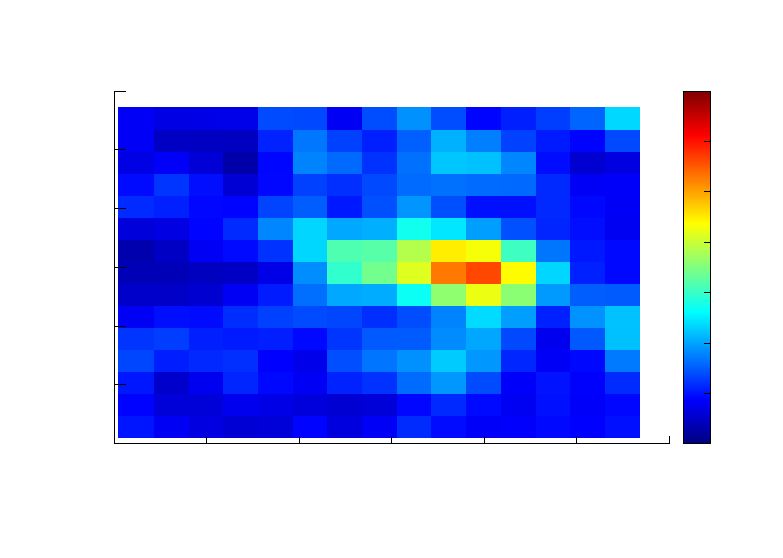
\includegraphics{plots/2DMRI600}}%
    \gplfronttext
  \end{picture}%
\endgroup
}
% \subcaptionbox{Es wurde als nächstes eine Polarisationszeit von $\SI{1300}{\milli\second}$ gewählt, wobei es sich hierbei um einen Wert zwischen den beiden Polarisationszeiten handelt.}
% {% GNUPLOT: LaTeX picture with Postscript
\begingroup
  % Encoding inside the plot.  In the header of your document, this encoding
  % should to defined, e.g., by using
  % \usepackage[cp1252,<other encodings>]{inputenc}
  \inputencoding{cp1252}%
  \makeatletter
  \providecommand\color[2][]{%
    \GenericError{(gnuplot) \space\space\space\@spaces}{%
      Package color not loaded in conjunction with
      terminal option `colourtext'%
    }{See the gnuplot documentation for explanation.%
    }{Either use 'blacktext' in gnuplot or load the package
      color.sty in LaTeX.}%
    \renewcommand\color[2][]{}%
  }%
  \providecommand\includegraphics[2][]{%
    \GenericError{(gnuplot) \space\space\space\@spaces}{%
      Package graphicx or graphics not loaded%
    }{See the gnuplot documentation for explanation.%
    }{The gnuplot epslatex terminal needs graphicx.sty or graphics.sty.}%
    \renewcommand\includegraphics[2][]{}%
  }%
  \providecommand\rotatebox[2]{#2}%
  \@ifundefined{ifGPcolor}{%
    \newif\ifGPcolor
    \GPcolorfalse
  }{}%
  \@ifundefined{ifGPblacktext}{%
    \newif\ifGPblacktext
    \GPblacktexttrue
  }{}%
  % define a \g@addto@macro without @ in the name:
  \let\gplgaddtomacro\g@addto@macro
  % define empty templates for all commands taking text:
  \gdef\gplbacktext{}%
  \gdef\gplfronttext{}%
  \makeatother
  \ifGPblacktext
    % no textcolor at all
    \def\colorrgb#1{}%
    \def\colorgray#1{}%
  \else
    % gray or color?
    \ifGPcolor
      \def\colorrgb#1{\color[rgb]{#1}}%
      \def\colorgray#1{\color[gray]{#1}}%
      \expandafter\def\csname LTw\endcsname{\color{white}}%
      \expandafter\def\csname LTb\endcsname{\color{black}}%
      \expandafter\def\csname LTa\endcsname{\color{black}}%
      \expandafter\def\csname LT0\endcsname{\color[rgb]{1,0,0}}%
      \expandafter\def\csname LT1\endcsname{\color[rgb]{0,1,0}}%
      \expandafter\def\csname LT2\endcsname{\color[rgb]{0,0,1}}%
      \expandafter\def\csname LT3\endcsname{\color[rgb]{1,0,1}}%
      \expandafter\def\csname LT4\endcsname{\color[rgb]{0,1,1}}%
      \expandafter\def\csname LT5\endcsname{\color[rgb]{1,1,0}}%
      \expandafter\def\csname LT6\endcsname{\color[rgb]{0,0,0}}%
      \expandafter\def\csname LT7\endcsname{\color[rgb]{1,0.3,0}}%
      \expandafter\def\csname LT8\endcsname{\color[rgb]{0.5,0.5,0.5}}%
    \else
      % gray
      \def\colorrgb#1{\color{black}}%
      \def\colorgray#1{\color[gray]{#1}}%
      \expandafter\def\csname LTw\endcsname{\color{white}}%
      \expandafter\def\csname LTb\endcsname{\color{black}}%
      \expandafter\def\csname LTa\endcsname{\color{black}}%
      \expandafter\def\csname LT0\endcsname{\color{black}}%
      \expandafter\def\csname LT1\endcsname{\color{black}}%
      \expandafter\def\csname LT2\endcsname{\color{black}}%
      \expandafter\def\csname LT3\endcsname{\color{black}}%
      \expandafter\def\csname LT4\endcsname{\color{black}}%
      \expandafter\def\csname LT5\endcsname{\color{black}}%
      \expandafter\def\csname LT6\endcsname{\color{black}}%
      \expandafter\def\csname LT7\endcsname{\color{black}}%
      \expandafter\def\csname LT8\endcsname{\color{black}}%
    \fi
  \fi
    \setlength{\unitlength}{0.0500bp}%
    \ifx\gptboxheight\undefined%
      \newlength{\gptboxheight}%
      \newlength{\gptboxwidth}%
      \newsavebox{\gptboxtext}%
    \fi%
    \setlength{\fboxrule}{0.5pt}%
    \setlength{\fboxsep}{1pt}%
\begin{picture}(7200.00,5040.00)%
    \gplgaddtomacro\gplbacktext{%
    }%
    \gplgaddtomacro\gplfronttext{%
      \csname LTb\endcsname%%
      \put(936,688){\makebox(0,0){\strut{}$0$}}%
      \put(1824,688){\makebox(0,0){\strut{}$20$}}%
      \put(2712,688){\makebox(0,0){\strut{}$40$}}%
      \put(3600,688){\makebox(0,0){\strut{}$60$}}%
      \put(4488,688){\makebox(0,0){\strut{}$80$}}%
      \put(5376,688){\makebox(0,0){\strut{}$100$}}%
      \put(6264,688){\makebox(0,0){\strut{}$120$}}%
      \put(3600,358){\makebox(0,0){\strut{}Y in $\si{\milli \meter}$}}%
      \put(700,938){\makebox(0,0)[r]{\strut{}$0$}}%
      \put(700,1502){\makebox(0,0)[r]{\strut{}$20$}}%
      \put(700,2066){\makebox(0,0)[r]{\strut{}$40$}}%
      \put(700,2630){\makebox(0,0)[r]{\strut{}$60$}}%
      \put(700,3194){\makebox(0,0)[r]{\strut{}$80$}}%
      \put(700,3758){\makebox(0,0)[r]{\strut{}$100$}}%
      \put(700,4322){\makebox(0,0)[r]{\strut{}$120$}}%
      \put(238,2630){\rotatebox{-270}{\makebox(0,0){\strut{}Z in $\si{\milli \meter}$}}}%
      \put(6795,938){\makebox(0,0)[l]{\strut{}$0$}}%
      \put(6795,1502){\makebox(0,0)[l]{\strut{}$10000$}}%
      \put(6795,2066){\makebox(0,0)[l]{\strut{}$20000$}}%
      \put(6795,2630){\makebox(0,0)[l]{\strut{}$30000$}}%
      \put(6795,3194){\makebox(0,0)[l]{\strut{}$40000$}}%
      \put(6795,3758){\makebox(0,0)[l]{\strut{}$50000$}}%
      \put(6795,4322){\makebox(0,0)[l]{\strut{}$60000$}}%
    }%
    \gplbacktext
    \put(0,0){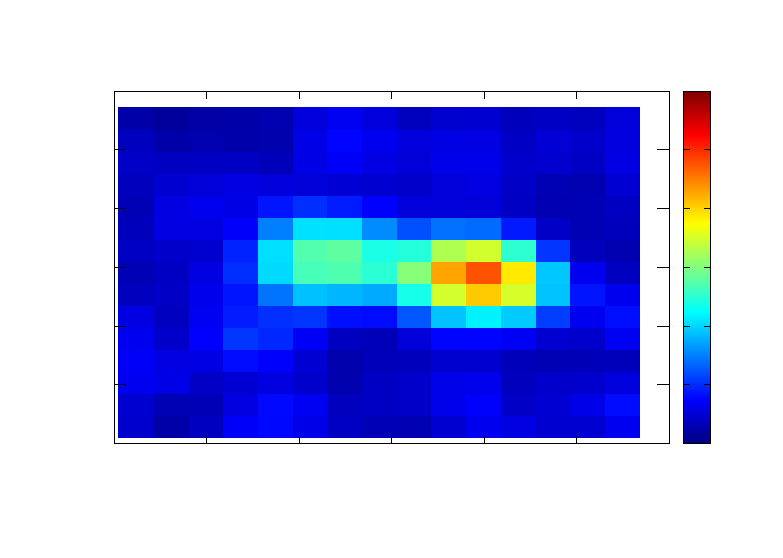
\includegraphics{plots/2DMRI1300}}%
    \gplfronttext
  \end{picture}%
\endgroup
}\newpage
\subcaptionbox{Im letzten Bild sollte eine Polarisationszeit doppelt so lange wie die längere $T_1$-Relaxation gewählt werden. Es wurde jedoch nur eine Polarisationszeit von $\SI{2800}{\milli\second}$ gemessen. Dabei handelt es sich um ca. das 1,5-fache der $T_1$-Zeit von der linken Röhre.}
{% GNUPLOT: LaTeX picture with Postscript
\begingroup
  % Encoding inside the plot.  In the header of your document, this encoding
  % should to defined, e.g., by using
  % \usepackage[cp1252,<other encodings>]{inputenc}
  \inputencoding{cp1252}%
  \makeatletter
  \providecommand\color[2][]{%
    \GenericError{(gnuplot) \space\space\space\@spaces}{%
      Package color not loaded in conjunction with
      terminal option `colourtext'%
    }{See the gnuplot documentation for explanation.%
    }{Either use 'blacktext' in gnuplot or load the package
      color.sty in LaTeX.}%
    \renewcommand\color[2][]{}%
  }%
  \providecommand\includegraphics[2][]{%
    \GenericError{(gnuplot) \space\space\space\@spaces}{%
      Package graphicx or graphics not loaded%
    }{See the gnuplot documentation for explanation.%
    }{The gnuplot epslatex terminal needs graphicx.sty or graphics.sty.}%
    \renewcommand\includegraphics[2][]{}%
  }%
  \providecommand\rotatebox[2]{#2}%
  \@ifundefined{ifGPcolor}{%
    \newif\ifGPcolor
    \GPcolorfalse
  }{}%
  \@ifundefined{ifGPblacktext}{%
    \newif\ifGPblacktext
    \GPblacktexttrue
  }{}%
  % define a \g@addto@macro without @ in the name:
  \let\gplgaddtomacro\g@addto@macro
  % define empty templates for all commands taking text:
  \gdef\gplbacktext{}%
  \gdef\gplfronttext{}%
  \makeatother
  \ifGPblacktext
    % no textcolor at all
    \def\colorrgb#1{}%
    \def\colorgray#1{}%
  \else
    % gray or color?
    \ifGPcolor
      \def\colorrgb#1{\color[rgb]{#1}}%
      \def\colorgray#1{\color[gray]{#1}}%
      \expandafter\def\csname LTw\endcsname{\color{white}}%
      \expandafter\def\csname LTb\endcsname{\color{black}}%
      \expandafter\def\csname LTa\endcsname{\color{black}}%
      \expandafter\def\csname LT0\endcsname{\color[rgb]{1,0,0}}%
      \expandafter\def\csname LT1\endcsname{\color[rgb]{0,1,0}}%
      \expandafter\def\csname LT2\endcsname{\color[rgb]{0,0,1}}%
      \expandafter\def\csname LT3\endcsname{\color[rgb]{1,0,1}}%
      \expandafter\def\csname LT4\endcsname{\color[rgb]{0,1,1}}%
      \expandafter\def\csname LT5\endcsname{\color[rgb]{1,1,0}}%
      \expandafter\def\csname LT6\endcsname{\color[rgb]{0,0,0}}%
      \expandafter\def\csname LT7\endcsname{\color[rgb]{1,0.3,0}}%
      \expandafter\def\csname LT8\endcsname{\color[rgb]{0.5,0.5,0.5}}%
    \else
      % gray
      \def\colorrgb#1{\color{black}}%
      \def\colorgray#1{\color[gray]{#1}}%
      \expandafter\def\csname LTw\endcsname{\color{white}}%
      \expandafter\def\csname LTb\endcsname{\color{black}}%
      \expandafter\def\csname LTa\endcsname{\color{black}}%
      \expandafter\def\csname LT0\endcsname{\color{black}}%
      \expandafter\def\csname LT1\endcsname{\color{black}}%
      \expandafter\def\csname LT2\endcsname{\color{black}}%
      \expandafter\def\csname LT3\endcsname{\color{black}}%
      \expandafter\def\csname LT4\endcsname{\color{black}}%
      \expandafter\def\csname LT5\endcsname{\color{black}}%
      \expandafter\def\csname LT6\endcsname{\color{black}}%
      \expandafter\def\csname LT7\endcsname{\color{black}}%
      \expandafter\def\csname LT8\endcsname{\color{black}}%
    \fi
  \fi
    \setlength{\unitlength}{0.0500bp}%
    \ifx\gptboxheight\undefined%
      \newlength{\gptboxheight}%
      \newlength{\gptboxwidth}%
      \newsavebox{\gptboxtext}%
    \fi%
    \setlength{\fboxrule}{0.5pt}%
    \setlength{\fboxsep}{1pt}%
\begin{picture}(7200.00,5040.00)%
    \gplgaddtomacro\gplbacktext{%
    }%
    \gplgaddtomacro\gplfronttext{%
      \csname LTb\endcsname%%
      \put(936,688){\makebox(0,0){\strut{}$0$}}%
      \put(1824,688){\makebox(0,0){\strut{}$20$}}%
      \put(2712,688){\makebox(0,0){\strut{}$40$}}%
      \put(3600,688){\makebox(0,0){\strut{}$60$}}%
      \put(4488,688){\makebox(0,0){\strut{}$80$}}%
      \put(5376,688){\makebox(0,0){\strut{}$100$}}%
      \put(6264,688){\makebox(0,0){\strut{}$120$}}%
      \put(3600,358){\makebox(0,0){\strut{}Y in $\si{\milli \meter}$}}%
      \put(700,938){\makebox(0,0)[r]{\strut{}$0$}}%
      \put(700,1502){\makebox(0,0)[r]{\strut{}$20$}}%
      \put(700,2066){\makebox(0,0)[r]{\strut{}$40$}}%
      \put(700,2630){\makebox(0,0)[r]{\strut{}$60$}}%
      \put(700,3194){\makebox(0,0)[r]{\strut{}$80$}}%
      \put(700,3758){\makebox(0,0)[r]{\strut{}$100$}}%
      \put(700,4322){\makebox(0,0)[r]{\strut{}$120$}}%
      \put(238,2630){\rotatebox{-270}{\makebox(0,0){\strut{}Z in $\si{\milli \meter}$}}}%
      \put(6795,938){\makebox(0,0)[l]{\strut{}$0$}}%
      \put(6795,1502){\makebox(0,0)[l]{\strut{}$10000$}}%
      \put(6795,2066){\makebox(0,0)[l]{\strut{}$20000$}}%
      \put(6795,2630){\makebox(0,0)[l]{\strut{}$30000$}}%
      \put(6795,3194){\makebox(0,0)[l]{\strut{}$40000$}}%
      \put(6795,3758){\makebox(0,0)[l]{\strut{}$50000$}}%
      \put(6795,4322){\makebox(0,0)[l]{\strut{}$60000$}}%
    }%
    \gplbacktext
    \put(0,0){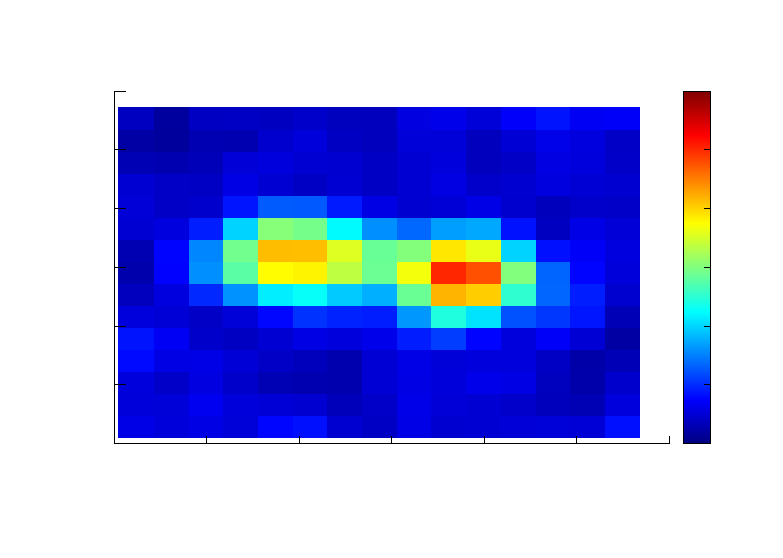
\includegraphics{plots/2DMRI2800}}%
    \gplfronttext
  \end{picture}%
\endgroup
}
\caption[Kontraste von $T_1$-Relaxation werden deutlich gemacht indem die Polarisationszeiten verändert werden]{Kontraste von $T_1$-Relaxation werden deutlich gemacht indem die Polarisationszeiten verändert werden. In Abb. (a) ist deutlich zu sehen, dass die Intensität rechts im Bild sehr groß ist. Hierbei kann auf eine kurze $T_1$-Zeit geschlossen werden, da die Spins sich in der rechten Röhre schon angefangen haben auszurichten und somit zum Signal beitragen. Bei längeren Polarisationszeiten ist zu erkennen, dass auch die Spins in der linken Röhre sich ausgerichtet haben und somit auch hier ein Signal detektiert werden kann. }\label{fig:11600}
\end{figure}
In der Abbildung \ref{fig:11600} wird eine Polarisationszeit von $\SI{600}{\milli\second}$ verwendet,
 welches die kürzere $T_1$-Zeit von der einen Röhre darstellt. Diese Röhre kann in Abb. \ref{fig:11600} unter anderem dadurch beobachtet werden,
dass sie durch eine starke Intensität dargestellt wird. Da diese Farbe von dem Rest hervorgehoben wird, wird dies als positives Kontrastmittel bezeichnet.
Die Intensitätsskalierung rechts von der Abbildung ist eine vom Programm kodierte Größe, die keine Einheit besitzt.\\

Warum die eine Röhre intensiver leuchtet als die andere, liegt am Zusammenhang zwischen der Polarisationszeit und der $T_1$-Relaxation. Die $T_1$-Relaxation gibt die Zeit an, bei der die meisten Spins sich dem äußeren Magnetfeld angepasst haben. Dies bedeutet, je kürzer $T_1$ ist, desto kürzer muss der Polarisationspuls sein um die meisten Spins im Material auszurichten. Wenn nun weiter gedacht wird und ein Material mit zwei $T_1$-Zeiten zur Untersuchung bereit stehen hat, so ist bei kleiner Polarisationszeit genau der Teil im Bild intensiver zu sehen, der eine kleinere $T_1$-Zeit besitzt, da in diesem Teil die meisten Spins sich schon ausgerichtet haben und dementsprechend zu dem MRI Signal beitragen können.\\
Durch Erhöhung der Polarisationszeit kann unteranderem auch die zweite Röhre sichtbar gemacht werden. Diese wird unter anderem in der Abb \ref{fig:11600} (b)  deutlich gemacht. Neben der Röhre die rechts unten im Bild vorhanden ist, ist hier auch die andere Röhre mit der größerer $T_1$-Zeit zu sehen. Hierbei sollte eine Polarisationszeit doppelt so groß wie die größere $T_1$-Zeit genommen werden, da in beiden Materialien versucht wird die ganzen Spins auszurichten. Am Versuchstag wurde sich mit einer Zeit von $\SI{2800}{\milli\second}$ zufrieden gegeben, da diese ausreichend zeigt, dass nun auch die zweite Röhre zu dem Signal beiträgt. Dennoch ist ein Kontrast zwischen den beiden Bildern zu sehen. Dies lässt darauf schließen, dass in der Röhre links in der Abbildung insgesamt weniger Spins vorhanden sind, die zu dem Signal beitragen und somit auch logischerweise die Intensität geringer ist. Womöglich ist ein anderer Grund, dass die Polarisationszeit nicht lange genug gewählt wurde, sodass hier nicht alle Spins ausgerichtet waren. Jedoch ist offensichtlich ein Unterschied zwischen den beiden Bildern sichtbar, welcher auch erklärt werden kann. Dies ist bei einer qualitativen Beobachtung das Wichtigste und somit genügen die zwei Abbildungen als Vergleich. Wenn zusätzlich noch eine Messung mit einer Polarisationszeit betrachtet wird, die sich zwischen den zwei $T_1$-Zeiten befindet, so müsste ein Teil von der einen Röhre schon sichtbar sein, jedoch dürfte die Intensität dieser Röhre geringer sein und somit einen bläulicheren Ton besitzten. Mit der Polarisationszeit von $\SI{1300}{\milli\second}$ wurde genau so eine Messung durchgeführt und in Abb \ref{fig: 1300} kann genau diese Vermutung beobachtet werden.
    \begin{figure}[H]
        \centering
        % GNUPLOT: LaTeX picture with Postscript
\begingroup
  % Encoding inside the plot.  In the header of your document, this encoding
  % should to defined, e.g., by using
  % \usepackage[cp1252,<other encodings>]{inputenc}
  \inputencoding{cp1252}%
  \makeatletter
  \providecommand\color[2][]{%
    \GenericError{(gnuplot) \space\space\space\@spaces}{%
      Package color not loaded in conjunction with
      terminal option `colourtext'%
    }{See the gnuplot documentation for explanation.%
    }{Either use 'blacktext' in gnuplot or load the package
      color.sty in LaTeX.}%
    \renewcommand\color[2][]{}%
  }%
  \providecommand\includegraphics[2][]{%
    \GenericError{(gnuplot) \space\space\space\@spaces}{%
      Package graphicx or graphics not loaded%
    }{See the gnuplot documentation for explanation.%
    }{The gnuplot epslatex terminal needs graphicx.sty or graphics.sty.}%
    \renewcommand\includegraphics[2][]{}%
  }%
  \providecommand\rotatebox[2]{#2}%
  \@ifundefined{ifGPcolor}{%
    \newif\ifGPcolor
    \GPcolorfalse
  }{}%
  \@ifundefined{ifGPblacktext}{%
    \newif\ifGPblacktext
    \GPblacktexttrue
  }{}%
  % define a \g@addto@macro without @ in the name:
  \let\gplgaddtomacro\g@addto@macro
  % define empty templates for all commands taking text:
  \gdef\gplbacktext{}%
  \gdef\gplfronttext{}%
  \makeatother
  \ifGPblacktext
    % no textcolor at all
    \def\colorrgb#1{}%
    \def\colorgray#1{}%
  \else
    % gray or color?
    \ifGPcolor
      \def\colorrgb#1{\color[rgb]{#1}}%
      \def\colorgray#1{\color[gray]{#1}}%
      \expandafter\def\csname LTw\endcsname{\color{white}}%
      \expandafter\def\csname LTb\endcsname{\color{black}}%
      \expandafter\def\csname LTa\endcsname{\color{black}}%
      \expandafter\def\csname LT0\endcsname{\color[rgb]{1,0,0}}%
      \expandafter\def\csname LT1\endcsname{\color[rgb]{0,1,0}}%
      \expandafter\def\csname LT2\endcsname{\color[rgb]{0,0,1}}%
      \expandafter\def\csname LT3\endcsname{\color[rgb]{1,0,1}}%
      \expandafter\def\csname LT4\endcsname{\color[rgb]{0,1,1}}%
      \expandafter\def\csname LT5\endcsname{\color[rgb]{1,1,0}}%
      \expandafter\def\csname LT6\endcsname{\color[rgb]{0,0,0}}%
      \expandafter\def\csname LT7\endcsname{\color[rgb]{1,0.3,0}}%
      \expandafter\def\csname LT8\endcsname{\color[rgb]{0.5,0.5,0.5}}%
    \else
      % gray
      \def\colorrgb#1{\color{black}}%
      \def\colorgray#1{\color[gray]{#1}}%
      \expandafter\def\csname LTw\endcsname{\color{white}}%
      \expandafter\def\csname LTb\endcsname{\color{black}}%
      \expandafter\def\csname LTa\endcsname{\color{black}}%
      \expandafter\def\csname LT0\endcsname{\color{black}}%
      \expandafter\def\csname LT1\endcsname{\color{black}}%
      \expandafter\def\csname LT2\endcsname{\color{black}}%
      \expandafter\def\csname LT3\endcsname{\color{black}}%
      \expandafter\def\csname LT4\endcsname{\color{black}}%
      \expandafter\def\csname LT5\endcsname{\color{black}}%
      \expandafter\def\csname LT6\endcsname{\color{black}}%
      \expandafter\def\csname LT7\endcsname{\color{black}}%
      \expandafter\def\csname LT8\endcsname{\color{black}}%
    \fi
  \fi
    \setlength{\unitlength}{0.0500bp}%
    \ifx\gptboxheight\undefined%
      \newlength{\gptboxheight}%
      \newlength{\gptboxwidth}%
      \newsavebox{\gptboxtext}%
    \fi%
    \setlength{\fboxrule}{0.5pt}%
    \setlength{\fboxsep}{1pt}%
\begin{picture}(7200.00,5040.00)%
    \gplgaddtomacro\gplbacktext{%
    }%
    \gplgaddtomacro\gplfronttext{%
      \csname LTb\endcsname%%
      \put(936,688){\makebox(0,0){\strut{}$0$}}%
      \put(1824,688){\makebox(0,0){\strut{}$20$}}%
      \put(2712,688){\makebox(0,0){\strut{}$40$}}%
      \put(3600,688){\makebox(0,0){\strut{}$60$}}%
      \put(4488,688){\makebox(0,0){\strut{}$80$}}%
      \put(5376,688){\makebox(0,0){\strut{}$100$}}%
      \put(6264,688){\makebox(0,0){\strut{}$120$}}%
      \put(3600,358){\makebox(0,0){\strut{}Y in $\si{\milli \meter}$}}%
      \put(700,938){\makebox(0,0)[r]{\strut{}$0$}}%
      \put(700,1502){\makebox(0,0)[r]{\strut{}$20$}}%
      \put(700,2066){\makebox(0,0)[r]{\strut{}$40$}}%
      \put(700,2630){\makebox(0,0)[r]{\strut{}$60$}}%
      \put(700,3194){\makebox(0,0)[r]{\strut{}$80$}}%
      \put(700,3758){\makebox(0,0)[r]{\strut{}$100$}}%
      \put(700,4322){\makebox(0,0)[r]{\strut{}$120$}}%
      \put(238,2630){\rotatebox{-270}{\makebox(0,0){\strut{}Z in $\si{\milli \meter}$}}}%
      \put(6795,938){\makebox(0,0)[l]{\strut{}$0$}}%
      \put(6795,1502){\makebox(0,0)[l]{\strut{}$10000$}}%
      \put(6795,2066){\makebox(0,0)[l]{\strut{}$20000$}}%
      \put(6795,2630){\makebox(0,0)[l]{\strut{}$30000$}}%
      \put(6795,3194){\makebox(0,0)[l]{\strut{}$40000$}}%
      \put(6795,3758){\makebox(0,0)[l]{\strut{}$50000$}}%
      \put(6795,4322){\makebox(0,0)[l]{\strut{}$60000$}}%
    }%
    \gplbacktext
    \put(0,0){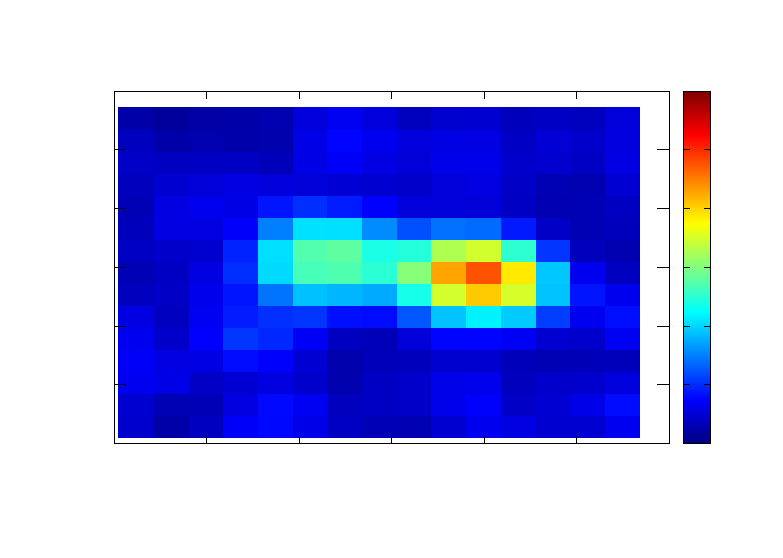
\includegraphics{plots/2DMRI1300}}%
    \gplfronttext
  \end{picture}%
\endgroup

        \caption[2D MRI mit der Polarisationszeit $\SI{1300}{\milli\second}$]{2D MRI mit der Polarisationszeit $\SI{1300}{\milli\second}$. Wie zu erwarten ist, ist das Signal in der linken Röhre noch nicht so intensiv wie in Abb. \ref{fig:11600} (b). Dies lässt sich dadurch erklären, dass die Polarisationszeit nicht komplett ausreicht um alle Spins schon auszurichten, jedoch aber einige Spins schon ausgerichtet wurden.}
        \label{fig: 1300}
    \end{figure}
Nun gibt es noch zwei verschiedene Sachen, die betrachtet werden können. Das erste was diskutiert werden muss ist, dass in der ersten Abb \ref{fig:11600} an manchen Stellen ein Signal vorhanden ist, wo keins sein dürfte. Somit wird außerhalb von dem Phantom ein Signal gemessen. Dies könnte unter anderem daran liegen, dass während des Messvorgang eine Matrixgröße von 64$\times$ 64 genommen wurde, sodass die Messzeit sehr lange gewesen ist. Diese wurde jedoch abgebrochen, weil diese zu lange gedauert hat und somit sind die Messdaten nicht vollständig, bzw. könnten wie bei einer anderen Datei beschädigt sein. Wenn nicht ausreichend Messpunkte genommen worden sind, kann es sein, dass die Auflösung nicht gut genug ist und somit das Phantom verschwommener dargestellt wird, was auch eine Ursache darstellen könnte.\\
Aus den Abbildungen kann entnommen werden, dass die Substanz in der rechten Röhre eine kleinere $T_1$-Relaxation hat als die Substanz in der linken Röhre.\\
In dem Abschnitt über die \glqq Relaxationszeiten von Wasser und Zusatzmitteln\grqq \, wurden verschiedene Konzentrationen von Stoffen untersucht auf die jeweiligen Relaxationszeiten. In der ersten Abbildung \ref{fig:11600} ist schon bei einer geringen Polarisationszeit die rechte Röhre deutlich zu sehen. Dies legt die Vermutung nahe, dass die Substanz in der  rechten Röhre eine $T_1$-Zeit besitzt, die bei ca. $\SI{600}{\milli\second}$ liegt. Mit dieser Vermutung kann aus der Tabelle \ref{tab:T1T2} entnommen werden, dass es sich hierbei um \ce{Cu2+} mit einer Konzentration von $\SI{500}{\micro\mole}$ oder 
$\SI{1000}{\micro\mole}$ handelt. Um dies genau zu ermitteln, müsste vor dem 2D-MRI 
eine $T_1$ Messung stattfinden, ohne dass sich in der anderen Röhre etwas befindet. Die Konzentration von $\SI{2000}{\micro\mole}$ wurde ausgeschlossen, da die Signalintensität noch leicht ansteigt, wenn die Polarisationszeit weiter erhöht wird. Dies spricht dafür, dass die Polarisationszeit von $\SI{600}{\milli\second}$ nicht komplett ausreicht um alle Spins auszurichten. Falls es kein Kupfer ist, kann es sich möglicherweise um \ce{Mn2+} handeln mit einer Konzentration von ca. $\SI{50}{\micro\mole}$. Die Begründug hierfür wären analog wie zum Kupfer. Weitere Stoffe oder Konzentrationen können nicht genauer betrachtet werden, da es hierfür keine Referenzwerte gibt.\\
Als nächstes kann eine Vermutung angestellt werden, was sich in der linken Röhre befindet. Hierbei wird erst bei höherer Polarisationszeit sichtbar, dass das Signal intensiver wird. Das Signal ist hierbei bei der letzten Messung am intensivsten. Der Wert, der hierfür am besten passt liefert Wasser mit einer Relaxationszeit von ca. $\SI{2200}{\milli\second}$. Alle anderen $T_1$-Zeiten würden schon früher durch die lange Polarisationszeiten erreicht werden, weshalb Kupfer und Mangan ausgeschlossen werden können.\\


Bei dem 2D-MRI wurden nicht nur die $T_1$-Konstraste angeschaut, sondern auch die unterschiedlichen Kontraste der $T_2$-Relaxationen. 

    \begin{figure}[H]
        \centering
        \subcaptionbox{$t_{echo}$=$\SI{250}{\milli\second}$}
        {% GNUPLOT: LaTeX picture with Postscript
\begingroup
  % Encoding inside the plot.  In the header of your document, this encoding
  % should to defined, e.g., by using
  % \usepackage[cp1252,<other encodings>]{inputenc}
  \inputencoding{cp1252}%
  \makeatletter
  \providecommand\color[2][]{%
    \GenericError{(gnuplot) \space\space\space\@spaces}{%
      Package color not loaded in conjunction with
      terminal option `colourtext'%
    }{See the gnuplot documentation for explanation.%
    }{Either use 'blacktext' in gnuplot or load the package
      color.sty in LaTeX.}%
    \renewcommand\color[2][]{}%
  }%
  \providecommand\includegraphics[2][]{%
    \GenericError{(gnuplot) \space\space\space\@spaces}{%
      Package graphicx or graphics not loaded%
    }{See the gnuplot documentation for explanation.%
    }{The gnuplot epslatex terminal needs graphicx.sty or graphics.sty.}%
    \renewcommand\includegraphics[2][]{}%
  }%
  \providecommand\rotatebox[2]{#2}%
  \@ifundefined{ifGPcolor}{%
    \newif\ifGPcolor
    \GPcolorfalse
  }{}%
  \@ifundefined{ifGPblacktext}{%
    \newif\ifGPblacktext
    \GPblacktexttrue
  }{}%
  % define a \g@addto@macro without @ in the name:
  \let\gplgaddtomacro\g@addto@macro
  % define empty templates for all commands taking text:
  \gdef\gplbacktext{}%
  \gdef\gplfronttext{}%
  \makeatother
  \ifGPblacktext
    % no textcolor at all
    \def\colorrgb#1{}%
    \def\colorgray#1{}%
  \else
    % gray or color?
    \ifGPcolor
      \def\colorrgb#1{\color[rgb]{#1}}%
      \def\colorgray#1{\color[gray]{#1}}%
      \expandafter\def\csname LTw\endcsname{\color{white}}%
      \expandafter\def\csname LTb\endcsname{\color{black}}%
      \expandafter\def\csname LTa\endcsname{\color{black}}%
      \expandafter\def\csname LT0\endcsname{\color[rgb]{1,0,0}}%
      \expandafter\def\csname LT1\endcsname{\color[rgb]{0,1,0}}%
      \expandafter\def\csname LT2\endcsname{\color[rgb]{0,0,1}}%
      \expandafter\def\csname LT3\endcsname{\color[rgb]{1,0,1}}%
      \expandafter\def\csname LT4\endcsname{\color[rgb]{0,1,1}}%
      \expandafter\def\csname LT5\endcsname{\color[rgb]{1,1,0}}%
      \expandafter\def\csname LT6\endcsname{\color[rgb]{0,0,0}}%
      \expandafter\def\csname LT7\endcsname{\color[rgb]{1,0.3,0}}%
      \expandafter\def\csname LT8\endcsname{\color[rgb]{0.5,0.5,0.5}}%
    \else
      % gray
      \def\colorrgb#1{\color{black}}%
      \def\colorgray#1{\color[gray]{#1}}%
      \expandafter\def\csname LTw\endcsname{\color{white}}%
      \expandafter\def\csname LTb\endcsname{\color{black}}%
      \expandafter\def\csname LTa\endcsname{\color{black}}%
      \expandafter\def\csname LT0\endcsname{\color{black}}%
      \expandafter\def\csname LT1\endcsname{\color{black}}%
      \expandafter\def\csname LT2\endcsname{\color{black}}%
      \expandafter\def\csname LT3\endcsname{\color{black}}%
      \expandafter\def\csname LT4\endcsname{\color{black}}%
      \expandafter\def\csname LT5\endcsname{\color{black}}%
      \expandafter\def\csname LT6\endcsname{\color{black}}%
      \expandafter\def\csname LT7\endcsname{\color{black}}%
      \expandafter\def\csname LT8\endcsname{\color{black}}%
    \fi
  \fi
    \setlength{\unitlength}{0.0500bp}%
    \ifx\gptboxheight\undefined%
      \newlength{\gptboxheight}%
      \newlength{\gptboxwidth}%
      \newsavebox{\gptboxtext}%
    \fi%
    \setlength{\fboxrule}{0.5pt}%
    \setlength{\fboxsep}{1pt}%
\begin{picture}(7200.00,5040.00)%
    \gplgaddtomacro\gplbacktext{%
    }%
    \gplgaddtomacro\gplfronttext{%
      \csname LTb\endcsname%%
      \put(936,688){\makebox(0,0){\strut{}$0$}}%
      \put(1824,688){\makebox(0,0){\strut{}$20$}}%
      \put(2712,688){\makebox(0,0){\strut{}$40$}}%
      \put(3600,688){\makebox(0,0){\strut{}$60$}}%
      \put(4488,688){\makebox(0,0){\strut{}$80$}}%
      \put(5376,688){\makebox(0,0){\strut{}$100$}}%
      \put(6264,688){\makebox(0,0){\strut{}$120$}}%
      \put(3600,358){\makebox(0,0){\strut{}Y in $\si{\milli \meter}$}}%
      \put(700,938){\makebox(0,0)[r]{\strut{}$0$}}%
      \put(700,1502){\makebox(0,0)[r]{\strut{}$20$}}%
      \put(700,2066){\makebox(0,0)[r]{\strut{}$40$}}%
      \put(700,2630){\makebox(0,0)[r]{\strut{}$60$}}%
      \put(700,3194){\makebox(0,0)[r]{\strut{}$80$}}%
      \put(700,3758){\makebox(0,0)[r]{\strut{}$100$}}%
      \put(700,4322){\makebox(0,0)[r]{\strut{}$120$}}%
      \put(238,2630){\rotatebox{-270}{\makebox(0,0){\strut{}Z in $\si{\milli \meter}$}}}%
      \put(6795,938){\makebox(0,0)[l]{\strut{}$0$}}%
      \put(6795,1421){\makebox(0,0)[l]{\strut{}$10000$}}%
      \put(6795,1904){\makebox(0,0)[l]{\strut{}$20000$}}%
      \put(6795,2388){\makebox(0,0)[l]{\strut{}$30000$}}%
      \put(6795,2871){\makebox(0,0)[l]{\strut{}$40000$}}%
      \put(6795,3355){\makebox(0,0)[l]{\strut{}$50000$}}%
      \put(6795,3838){\makebox(0,0)[l]{\strut{}$60000$}}%
      \put(6795,4322){\makebox(0,0)[l]{\strut{}$70000$}}%
    }%
    \gplbacktext
    \put(0,0){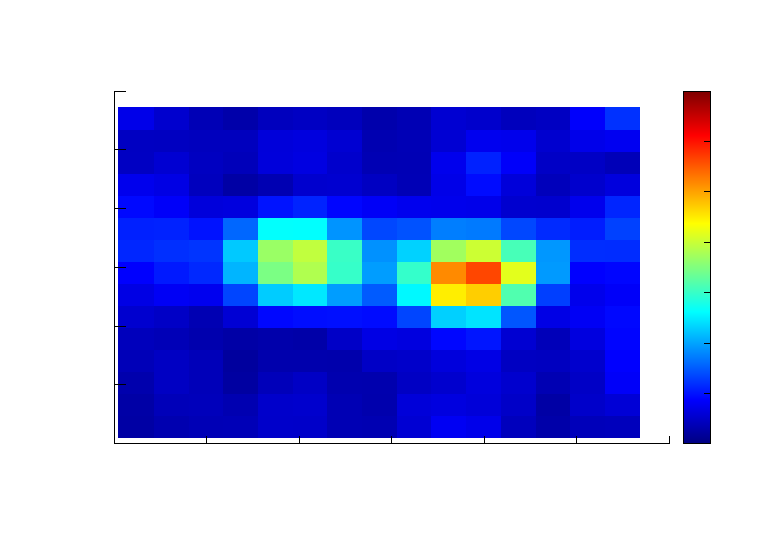
\includegraphics{plots/2DMRI250}}%
    \gplfronttext
  \end{picture}%
\endgroup
}
        \subcaptionbox{$t_{echo}$=$\SI{550}{\milli\second}$}
        {% GNUPLOT: LaTeX picture with Postscript
\begingroup
  % Encoding inside the plot.  In the header of your document, this encoding
  % should to defined, e.g., by using
  % \usepackage[cp1252,<other encodings>]{inputenc}
  \inputencoding{cp1252}%
  \makeatletter
  \providecommand\color[2][]{%
    \GenericError{(gnuplot) \space\space\space\@spaces}{%
      Package color not loaded in conjunction with
      terminal option `colourtext'%
    }{See the gnuplot documentation for explanation.%
    }{Either use 'blacktext' in gnuplot or load the package
      color.sty in LaTeX.}%
    \renewcommand\color[2][]{}%
  }%
  \providecommand\includegraphics[2][]{%
    \GenericError{(gnuplot) \space\space\space\@spaces}{%
      Package graphicx or graphics not loaded%
    }{See the gnuplot documentation for explanation.%
    }{The gnuplot epslatex terminal needs graphicx.sty or graphics.sty.}%
    \renewcommand\includegraphics[2][]{}%
  }%
  \providecommand\rotatebox[2]{#2}%
  \@ifundefined{ifGPcolor}{%
    \newif\ifGPcolor
    \GPcolorfalse
  }{}%
  \@ifundefined{ifGPblacktext}{%
    \newif\ifGPblacktext
    \GPblacktexttrue
  }{}%
  % define a \g@addto@macro without @ in the name:
  \let\gplgaddtomacro\g@addto@macro
  % define empty templates for all commands taking text:
  \gdef\gplbacktext{}%
  \gdef\gplfronttext{}%
  \makeatother
  \ifGPblacktext
    % no textcolor at all
    \def\colorrgb#1{}%
    \def\colorgray#1{}%
  \else
    % gray or color?
    \ifGPcolor
      \def\colorrgb#1{\color[rgb]{#1}}%
      \def\colorgray#1{\color[gray]{#1}}%
      \expandafter\def\csname LTw\endcsname{\color{white}}%
      \expandafter\def\csname LTb\endcsname{\color{black}}%
      \expandafter\def\csname LTa\endcsname{\color{black}}%
      \expandafter\def\csname LT0\endcsname{\color[rgb]{1,0,0}}%
      \expandafter\def\csname LT1\endcsname{\color[rgb]{0,1,0}}%
      \expandafter\def\csname LT2\endcsname{\color[rgb]{0,0,1}}%
      \expandafter\def\csname LT3\endcsname{\color[rgb]{1,0,1}}%
      \expandafter\def\csname LT4\endcsname{\color[rgb]{0,1,1}}%
      \expandafter\def\csname LT5\endcsname{\color[rgb]{1,1,0}}%
      \expandafter\def\csname LT6\endcsname{\color[rgb]{0,0,0}}%
      \expandafter\def\csname LT7\endcsname{\color[rgb]{1,0.3,0}}%
      \expandafter\def\csname LT8\endcsname{\color[rgb]{0.5,0.5,0.5}}%
    \else
      % gray
      \def\colorrgb#1{\color{black}}%
      \def\colorgray#1{\color[gray]{#1}}%
      \expandafter\def\csname LTw\endcsname{\color{white}}%
      \expandafter\def\csname LTb\endcsname{\color{black}}%
      \expandafter\def\csname LTa\endcsname{\color{black}}%
      \expandafter\def\csname LT0\endcsname{\color{black}}%
      \expandafter\def\csname LT1\endcsname{\color{black}}%
      \expandafter\def\csname LT2\endcsname{\color{black}}%
      \expandafter\def\csname LT3\endcsname{\color{black}}%
      \expandafter\def\csname LT4\endcsname{\color{black}}%
      \expandafter\def\csname LT5\endcsname{\color{black}}%
      \expandafter\def\csname LT6\endcsname{\color{black}}%
      \expandafter\def\csname LT7\endcsname{\color{black}}%
      \expandafter\def\csname LT8\endcsname{\color{black}}%
    \fi
  \fi
    \setlength{\unitlength}{0.0500bp}%
    \ifx\gptboxheight\undefined%
      \newlength{\gptboxheight}%
      \newlength{\gptboxwidth}%
      \newsavebox{\gptboxtext}%
    \fi%
    \setlength{\fboxrule}{0.5pt}%
    \setlength{\fboxsep}{1pt}%
\begin{picture}(7200.00,5040.00)%
    \gplgaddtomacro\gplbacktext{%
    }%
    \gplgaddtomacro\gplfronttext{%
      \csname LTb\endcsname%%
      \put(936,688){\makebox(0,0){\strut{}$0$}}%
      \put(1824,688){\makebox(0,0){\strut{}$20$}}%
      \put(2712,688){\makebox(0,0){\strut{}$40$}}%
      \put(3600,688){\makebox(0,0){\strut{}$60$}}%
      \put(4488,688){\makebox(0,0){\strut{}$80$}}%
      \put(5376,688){\makebox(0,0){\strut{}$100$}}%
      \put(6264,688){\makebox(0,0){\strut{}$120$}}%
      \put(3600,358){\makebox(0,0){\strut{}Y in $\si{\milli \meter}$}}%
      \put(700,938){\makebox(0,0)[r]{\strut{}$0$}}%
      \put(700,1502){\makebox(0,0)[r]{\strut{}$20$}}%
      \put(700,2066){\makebox(0,0)[r]{\strut{}$40$}}%
      \put(700,2630){\makebox(0,0)[r]{\strut{}$60$}}%
      \put(700,3194){\makebox(0,0)[r]{\strut{}$80$}}%
      \put(700,3758){\makebox(0,0)[r]{\strut{}$100$}}%
      \put(700,4322){\makebox(0,0)[r]{\strut{}$120$}}%
      \put(238,2630){\rotatebox{-270}{\makebox(0,0){\strut{}Z in $\si{\milli \meter}$}}}%
      \put(6795,938){\makebox(0,0)[l]{\strut{}$0$}}%
      \put(6795,1314){\makebox(0,0)[l]{\strut{}$5000$}}%
      \put(6795,1690){\makebox(0,0)[l]{\strut{}$10000$}}%
      \put(6795,2066){\makebox(0,0)[l]{\strut{}$15000$}}%
      \put(6795,2442){\makebox(0,0)[l]{\strut{}$20000$}}%
      \put(6795,2818){\makebox(0,0)[l]{\strut{}$25000$}}%
      \put(6795,3194){\makebox(0,0)[l]{\strut{}$30000$}}%
      \put(6795,3570){\makebox(0,0)[l]{\strut{}$35000$}}%
      \put(6795,3946){\makebox(0,0)[l]{\strut{}$40000$}}%
      \put(6795,4322){\makebox(0,0)[l]{\strut{}$45000$}}%
    }%
    \gplbacktext
    \put(0,0){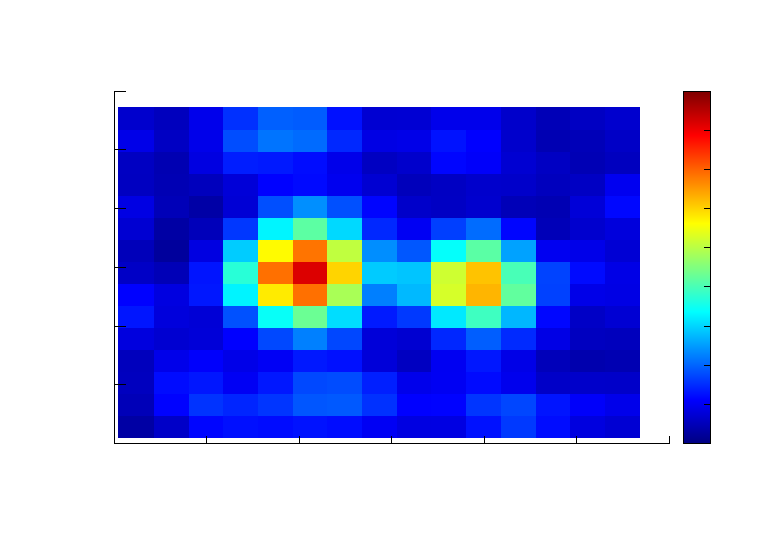
\includegraphics{plots/2DMRI550}}%
    \gplfronttext
  \end{picture}%
\endgroup
}
        \caption[2D-MRI mit Relaxationskontrast von verschiedenen $T_2$-Zeiten, durch verschiedene Echozeiten]{2D-MRI mit Relaxationskontrast von verschiedenen $T_2$-Zeiten, durch verschiedene Echozeiten deutlich gemacht. Im ersten Bild (a) kann beobachtet werden, dass bei geringer Echozeit die Spins nocht nicht relaxieren konnten und das Signal noch bei beiden Röhren relativ stark ist und fast die genaue Intensität wie in \ref{fig:11600}(b) besitzten. Bei längerer Echozeit wird der Kontrast von den zwei Röhren deutlicher. Je kürzer $T_2$ ist, desto schneller verschwindet die Intensität bei längeren Echozeiten. Somit kann aus dem zweiten Bild entnommen werden, dass die linke Röhre eine längere $T_2$-Zeit hat und somitrastmittl als ein positives Kont}\label{fig:1250}
    \end{figure}
Was als erstes auffält ist, dass die Abb. \ref{fig:1250} der Abb \ref{fig:11600}  vergleichsweise sehr ähnlich aussiehen. Dies liegt daran, dass bei der $T_2$-Realaxation der Kontrast mit der Zeit größer wird. (Bis zu dem Punkt wo beide keine Signale mehr besitzen) . Außerdem wurde hier auch die gleiche Polarisationszeit genommen, damit keine Unterschiede von der $T_1$-Relaxation die $T_2$-Kontraste beeinflussen. \\
Grund dafür, dass die $T_2$-Kontraste noch nicht so gut sichtbar sind liegt daran, dass bei kurzer Echozeit die Spins noch nicht stark relaxieren konnten und somit auch kein großer Unterschied im Signal vorhanden ist. Dies ändert sich jedoch mit der Messung \ref{fig:1250}, da hier das Signal von der rechten Röhre schwächer ist als in der linken Röhre. Zu beachten ist hierbei, dass die Skala sich auf der rechten Seite verändert hat und auch wenn das Signal in der linken Röhre mit rot ausgeprägt ist, dass dieses Signal leztlich auch schwächer geworden sind. Dies kann dadurch erklärt werden, dass die $T_2$-Relaxation die Zeit angibt, wie schnell ein Signal zerfällt. Dadurch, dass das Signal in der linken Röhre stärker als in der rechten Röhre zu sehen ist, handelt es sich hier um ein positives Kontrastmittel und die Substanz in der linken Röhre muss eine längere $T_2$-Relaxation besitzten.  
Dies würde auch mit der Theorie übereinstimmen, dass in der linken Röhre Wasser als Probe genommen wurde. Denn bei Wasser ist $T_2$ mit  $\SI{1901}{\milli\second}$ am größten und somit sollte das Signal auch bei längeren Echozeiten deutlicher zu sehen sein als bei Kupfer oder Mangan.
Schon in dem Kapitel davor \ref{sec:1DMRIkapitel} wurde darauf eingegangen, dass eine gute Effizienz wichtig ist, um bei einer geringen Messzeit eine gute Auflösung zu erhalten. Im zweidimensionalen wird dies um so wichtiger sein, da statt nur in eine Richtung nun eine zweite Richtung abgefahren wird, womit sich die Messzeit erheblich erhöht. Somit ist es wichtig bei dem Versuch darauf zu achten, dass die Effizienz gut ist.